%%%%%%%%%%%%%%%%%%%%%%%%%%%%%%%%%%%%%%%%%%%%%%%%%%%%%%%%%%%%%%%%%%%%%%%%%%%%%
%%
%% Classes disponibles :
%%	- times : utilisation de la police Times par défaut.
%%	- these, sujthese, projthese, memoire, essai, rapport : pour
%%		générer la page de garde en fonction du type document.
%%	- french, english : selon la langue dans laquelle doit
%%		être rédigé le document.
%%  - ieee, apa : style des références bibliographiques
%%  - twoside : alternance des marges pour impression recto/verso
%%    vous devez décommenter la ligne 22 si vous utilisez cette classe
%%
%%%%%%%%%%%%%%%%%%%%%%%%%%%%%%%%%%%%%%%%%%%%%%%%%%%%%%%%%%%%%%%%%%%%%%%%%%%%%%
\documentclass[12pt,times,rapport,french,apa]{uqac}

%%%%%%%%%%%%%%%%%%%%%%%%%%%%%%%%%%%%%%%%%%%%%%%%%%%%%%%
%%
%% Décommenter la ligne suivante avec l'utilisation de
%% la classe "twoside"
%%
%%%%%%%%%%%%%%%%%%%%%%%%%%%%%%%%%%%%%%%%%%%%%%%%%%%%%%%
% \raggedbottom

%%%%%%%%%%%%%%%%%%%%%%%%%%%%%%%%%%%%%
%%
%% Préciser l'emplacement du fichier
%% contenant les acronymes.
%%
%%%%%%%%%%%%%%%%%%%%%%%%%%%%%%%%%%%%%
\acrolistpath{assets/acro}

%%%%%%%%%%%%%%%%%%%%%%%%%%%%%%%%%%%%%%%%%%%%%%%%%%%%%%%%
%%
%% Toutes les images utilisées doivent se trouver dans
%% le répertoire "assets/figure".
%%
%%%%%%%%%%%%%%%%%%%%%%%%%%%%%%%%%%%%%%%%%%%%%%%%%%%%%%%%
\graphicspath{{assets/figures/}}

%%%%%%%%%%%%%%%%%%%%%%%%%%%%%%%%%%%%
%%
%% Packages utilisateurs ci-dessous:
%%
%%%%%%%%%%%%%%%%%%%%%%%%%%%%%%%%%%%%
\usepackage{color, xcolor, soulutf8}
\usepackage{tikz}
\usetikzlibrary{babel}
\usepackage{chemfig}
\usepackage{chemnum}
\usepackage[europeanresistors,americaninductors]{circuitikz}
\usepackage{tikz-feynman}
\usepackage{hyperref}
\hypersetup{
  colorlinks=true,
  linkcolor=black,
  urlcolor=[rgb]{0,0.501,0.674},
  breaklinks=true,
  citecolor=[rgb]{0,0.501,0.674},
  bookmarks=true
}

%%%%%%%%%%%%%%%%%%%%%
%%
%% Césures manuelles
%%
%%%%%%%%%%%%%%%%%%%%%
% \hyphenation{con-nection con-nue con-cep-tion}

%%%%%%%%%%%%%%%%%%%%%%%%%%%%%%%%
%%
%% Gestion des lignes orphelines
%%
%%%%%%%%%%%%%%%%%%%%%%%%%%%%%%%%
\widowpenalty10000
\clubpenalty10000

\begin{document}
\pagestyle{empty}
\thispagestyle{empty}

%%%%%%%%%%%%%%%%%%%%%%%%%%%%%
%%
%% Titre, auteur et programme
%%
%%%%%%%%%%%%%%%%%%%%%%%%%%%%%

\title{Système de détection d'anomalies et de gestion de logs pour la sécurité des réseaux}
\author{Larzul Julien}
\programme{Informatique}

%%%%%%%%%%%%%%%%%%%%%%%%%%%%%%%%%%%%%
%%
%% S’il y a lieu, indiquer le profil
%% ou la concentration du programme
%%
%%%%%%%%%%%%%%%%%%%%%%%%%%%%%%%%%%%%%
%\concentration{profil recherche}

%%%%%%%%%%%%%%%%%%%%%%%%%%%%%%%%%%%%%%%%%%%%
%%
%% Par défaut l'année courante est utilisée.
%% Pour spécifier une autre année :
%%
%%%%%%%%%%%%%%%%%%%%%%%%%%%%%%%%%%%%%%%%%%%%
%\degreeyear{2018}

\maketitle

%%%%%%%%%%%%%%%%%%%%%
%%
%% Page préliminaires
%%
%%%%%%%%%%%%%%%%%%%%%
\opening
% \pagestyle{empty}

% \begin{abstract}

Lorem ipsum dolor sit amet, consectetur adipisicing elit, sed do eiusmod
tempor incididunt ut labore et dolore magna aliqua. Ut enim ad minim veniam,
quis nostrud exercitation ullamco laboris nisi ut aliquip ex ea commodo
consequat. Duis aute irure dolor in reprehenderit in voluptate velit esse
cillum dolore eu fugiat nulla pariatur. Excepteur sint occaecat cupidatat non
proident, sunt in culpa qui officia deserunt mollit anim id est laborum.

Lorem ipsum dolor sit amet, consectetur adipisicing elit, sed do eiusmod
tempor incididunt ut labore et dolore magna aliqua. Ut enim ad minim veniam,
quis nostrud exercitation ullamco laboris nisi ut aliquip ex ea commodo
consequat. Duis aute irure dolor in reprehenderit in voluptate velit esse
cillum dolore eu fugiat nulla pariatur. Excepteur sint occaecat cupidatat non
proident, sunt in culpa qui officia deserunt mollit anim id est laborum.

\end{abstract}


%%%%%%%%%%%%%%%%%%%%%%%%%%%%%%%%%%%%%%%%%%%%%%%%%%%%%%%%%%
%%
%% Si vous écrivez un document en anglais,
%% il sera nécessaire de fournir un résumé en Français :
%%
%%%%%%%%%%%%%%%%%%%%%%%%%%%%%%%%%%%%%%%%%%%%%%%%%%%%%%%%%%
%\begin{resume}

Lorem ipsum dolor sit amet, consectetur adipisicing elit, sed do eiusmod
tempor incididunt ut labore et dolore magna aliqua. Ut enim ad minim veniam,
quis nostrud exercitation ullamco laboris nisi ut aliquip ex ea commodo
consequat. Duis aute irure dolor in reprehenderit in voluptate velit esse
cillum dolore eu fugiat nulla pariatur. Excepteur sint occaecat cupidatat non
proident, sunt in culpa qui officia deserunt mollit anim id est laborum.

Lorem ipsum dolor sit amet, consectetur adipisicing elit, sed do eiusmod
tempor incididunt ut labore et dolore magna aliqua. Ut enim ad minim veniam,
quis nostrud exercitation ullamco laboris nisi ut aliquip ex ea commodo
consequat. Duis aute irure dolor in reprehenderit in voluptate velit esse
cillum dolore eu fugiat nulla pariatur. Excepteur sint occaecat cupidatat non
proident, sunt in culpa qui officia deserunt mollit anim id est laborum.

\end{resume}


\tableofcontents
\cleardoublepage
% \listoftables
\listoffigures
% \listofacro

% \begin{dedic}

Lorem ipsum dolor sit amet, consectetur adipisicing elit, sed do eiusmod
tempor incididunt ut labore et dolore magna aliqua. Ut enim ad minim veniam,
quis nostrud exercitation ullamco laboris nisi ut aliquip ex ea commodo
consequat. Duis aute irure dolor in reprehenderit in voluptate velit esse
cillum dolore eu fugiat nulla pariatur. Excepteur sint occaecat cupidatat non
proident, sunt in culpa qui officia deserunt mollit anim id est laborum.

\end{dedic}

% \begin{ack}

Lorem ipsum dolor sit amet, consectetur adipisicing elit, sed do eiusmod
tempor incididunt ut labore et dolore magna aliqua. Ut enim ad minim veniam,
quis nostrud exercitation ullamco laboris nisi ut aliquip ex ea commodo
consequat. Duis aute irure dolor in reprehenderit in voluptate velit esse
cillum dolore eu fugiat nulla pariatur. Excepteur sint occaecat cupidatat non
proident, sunt in culpa qui officia deserunt mollit anim id est laborum.

Lorem ipsum dolor sit amet, consectetur adipisicing elit, sed do eiusmod
tempor incididunt ut labore et dolore magna aliqua. Ut enim ad minim veniam,
quis nostrud exercitation ullamco laboris nisi ut aliquip ex ea commodo
consequat. Duis aute irure dolor in reprehenderit in voluptate velit esse
cillum dolore eu fugiat nulla pariatur. Excepteur sint occaecat cupidatat non
proident, sunt in culpa qui officia deserunt mollit anim id est laborum.

\end{ack}

% \begin{preface}

Lorem ipsum dolor sit amet, consectetur adipisicing elit, sed do eiusmod
tempor incididunt ut labore et dolore magna aliqua. Ut enim ad minim veniam,
quis nostrud exercitation ullamco laboris nisi ut aliquip ex ea commodo
consequat. Duis aute irure dolor in reprehenderit in voluptate velit esse
cillum dolore eu fugiat nulla pariatur. Excepteur sint occaecat cupidatat non
proident, sunt in culpa qui officia deserunt mollit anim id est laborum.

Lorem ipsum dolor sit amet, consectetur adipisicing elit, sed do eiusmod
tempor incididunt ut labore et dolore magna aliqua. Ut enim ad minim veniam,
quis nostrud exercitation ullamco laboris nisi ut aliquip ex ea commodo
consequat. Duis aute irure dolor in reprehenderit in voluptate velit esse
cillum dolore eu fugiat nulla pariatur. Excepteur sint occaecat cupidatat non
proident, sunt in culpa qui officia deserunt mollit anim id est laborum.

\end{preface}


%%%%%%%%%%%%%%%%%%%%%
%%
%% Document principal
%%
%%%%%%%%%%%%%%%%%%%%%
% \pagestyle{fancy}
\maincontent

\begin{introduction}

Dans ce contexte, ce projet a pour objectif la conception et le déploiement d’un
\textit{système de détection d’anomalies et de gestion de logs}. 
L’approche consiste à mettre en place une chaîne complète allant de la collecte des journaux
jusqu’à leur visualisation et leur analyse via une interface conviviale. 
L’architecture retenue repose sur quatre briques logicielles complémentaires :
\begin{itemize}
    \item \textbf{Suricata}, un système de détection d’intrusions (IDS/IPS) chargé
    d’analyser le trafic réseau et de générer des alertes en temps réel ;
    \item \textbf{syslog-ng}, utilisé pour centraliser les journaux du système et des applications ;
    \item \textbf{Elasticsearch}, base de données NoSQL permettant l’indexation et la recherche rapide
    des événements collectés ;
    \item \textbf{Kibana}, une interface web offrant des fonctionnalités de visualisation et de
    création de tableaux de bord.
\end{itemize}

Le projet doit également inclure l’implémentation de plusieurs scénarios d’attaque
simulés. Ces cas d’intrusion permettront de valider la capacité du système à détecter
différents comportements malveillants et à générer des alertes exploitables par
l’administrateur.

Ce rapport présente dans un premier temps l’environnement mis en place et les choix
technologiques retenus. Il détaille ensuite la configuration et l’intégration des outils,
avant de décrire et d’analyser cinq scénarios d’intrusion représentatifs. 
Enfin, une partie est consacrée à la visualisation des résultats, à l’évaluation des limites
du système et aux perspectives d’amélioration.

\end{introduction}

\chapter{Présentation de l’architecture}
\label{chap:chap_1}

\chapter{Configuration et intégration}
\label{chap:chap_2}

\section{Configuration de Suricata}

\subsection{Vérification du chemin des règles}
Pour commencer, nous avons vérifié que le fichier \texttt{/etc/suricata/suricata.yaml} pointe bien vers le répertoire \texttt{/var/lib/suricata/rules}, et que le fichier \texttt{local.rules} est inclus dans la section \texttt{rule-files} :

\begin{verbatim}
$ grep -n "default-rule-path" /etc/suricata/suricata.yaml
2174:default-rule-path: /var/lib/suricata/rules

$ grep -A3 "rule-files:" /etc/suricata/suricata.yaml
2176:rule-files:
2177:  - suricata.rules
2178:  - local.rules
\end{verbatim}

\begin{figure}[H]
    \centering
    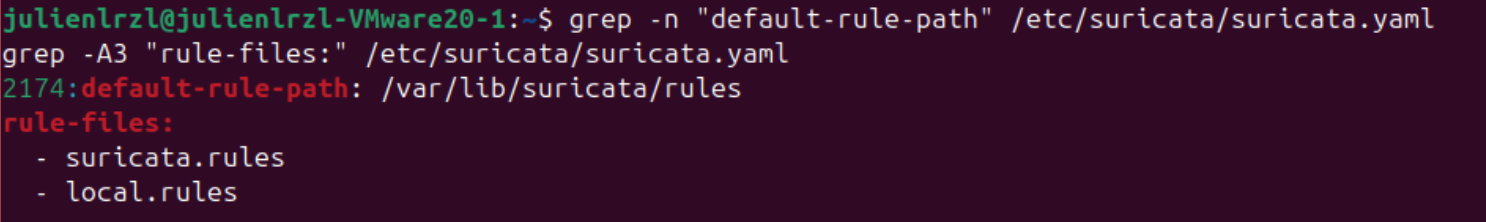
\includegraphics[width=0.9\linewidth]{assets/figures/suricata-rulefiles.png}
    \caption{Vérification du chemin des règles et inclusion de \texttt{local.rules}.}
\end{figure}

\subsection{Ajout d'une règle locale}
Une règle de détection ICMP a été ajoutée dans le fichier \texttt{local.rules} :

\begin{verbatim}
alert icmp any any -> any any (msg:"ICMP test detected"; sid:1000001; rev:1;)
\end{verbatim}


\begin{figure}[H]
    \centering
    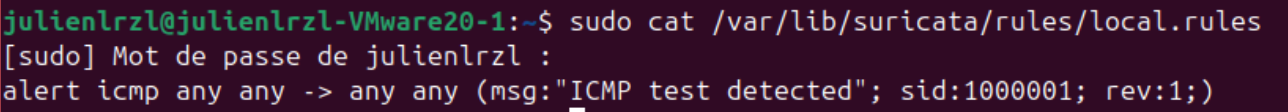
\includegraphics[width=0.9\linewidth]{assets/figures/local-rules.png}
    \caption{Règle ICMP de test ajoutée au fichier \texttt{local.rules}.}
\end{figure}

\subsection{Test de configuration}
Un test de configuration a permis de vérifier que le fichier YAML est valide et que les règles sont correctement chargées :

\begin{verbatim}
$ sudo suricata -T -c /etc/suricata/suricata.yaml
-- Configuration OK --
\end{verbatim}

\begin{figure}[H]
    \centering
    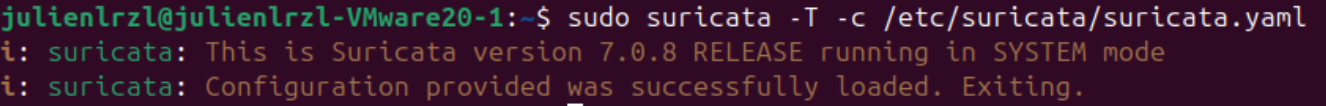
\includegraphics[width=0.9\linewidth]{assets/figures/suricata-test.png}
    \caption{Validation de la configuration de Suricata.}
\end{figure}

\subsection{Relance du service}
Suricata a ensuite été relancé en mode démon :

\begin{verbatim}
$ sudo pkill -9 suricata 2>/dev/null || true
$ sudo rm -f /var/run/suricata.pid
$ sudo suricata -c /etc/suricata/suricata.yaml -i ens160 -D
\end{verbatim}

\begin{figure}[H]
    \centering
    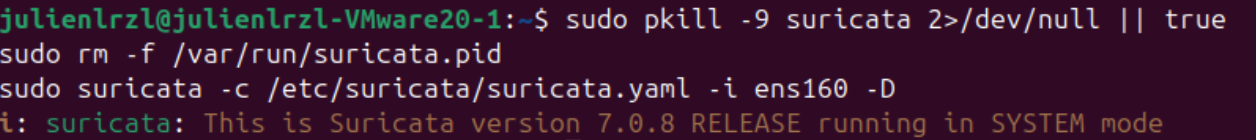
\includegraphics[width=0.9\linewidth]{assets/figures/suricata-restart.png}
    \caption{Relance de Suricata en mode démon sur l'interface \texttt{ens160}.}
\end{figure}

\subsection{Génération de trafic ICMP}
Un simple ping vers l’adresse publique de Google (8.8.8.8) a été utilisé pour générer du trafic ICMP :

\begin{verbatim}
$ ping -c 3 8.8.8.8
\end{verbatim}

\begin{figure}[H]
    \centering
    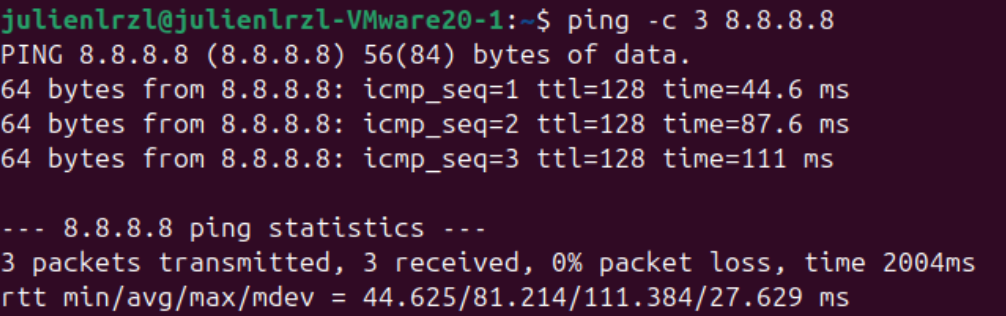
\includegraphics[width=0.9\linewidth]{assets/figures/ping-icmp.png}
    \caption{Génération de trafic ICMP avec la commande \texttt{ping}.}
\end{figure}

\subsection{Vérification des alertes générées}
L’analyse du fichier \texttt{/var/log/suricata/fast.log} montre bien que la règle locale a déclenché une alerte pour les paquets ICMP observés :

\begin{lstlisting}[style=bashstyle]
09/25/2025-18:16:40.523467 [**] [1:1000001:1] ICMP test detected [**] {ICMP} 172.16.150.130:8 -> 8.8.8.8:0
\end{lstlisting}


\begin{figure}[H]
    \centering
    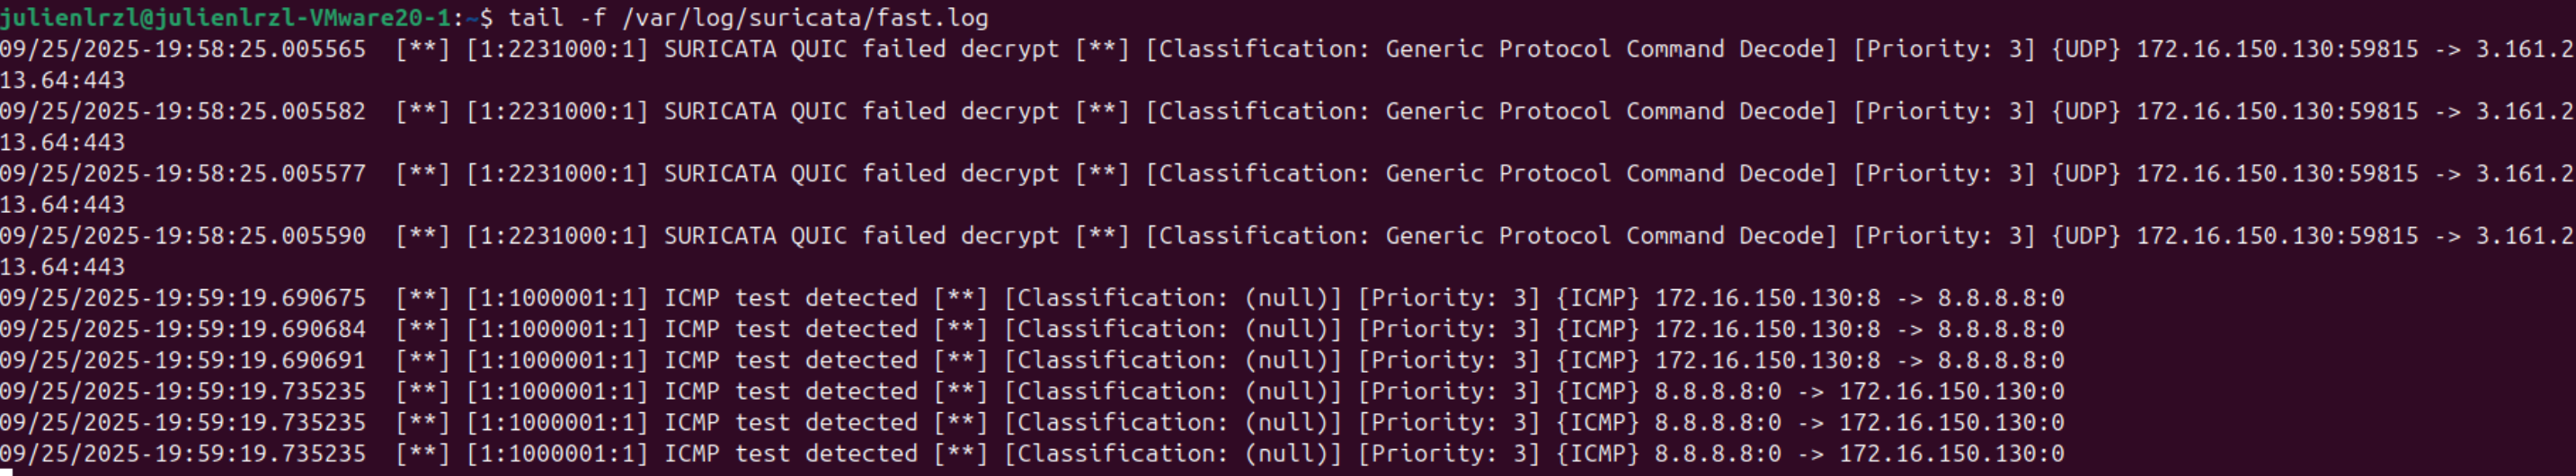
\includegraphics[width=0.9\linewidth]{assets/figures/icmp-alert.png}
    \caption{Alerte générée dans \texttt{fast.log} suite au ping ICMP.}
\end{figure}

\bigskip
En conclusion, Suricata est correctement configuré pour charger les règles locales et détecter du trafic ICMP simple, démontrant sa capacité à identifier des anomalies sur le réseau.
\chapter{Configuration et intégration}
\label{chap:chap_3}

\chapter{Visualisation et alertes}
\label{chap:chap_4}

\chapter{Visualisation et alertes}
\label{chap:chap_4}
\chapter{Analyse et discussion}
\label{chap:chap_4}
\begin{conclusion}



\end{conclusion}



%%%%%%%%$%%%%
%%
%% Références
%%
%%%%%%%%%%%%%

%%%%%%%%%%%%%%%%%%%%%%%%%%%%%%%%%%%%%%%%%%%%%%%%%%%%%%%%%%
%%
%% Le fichier BibTeX contenant les références
%% doit se trouver dans le répertoire "assets/references".
%%
%%%%%%%%%%%%%%%%%%%%%%%%%%%%%%%%%%%%%%%%%%%%%%%%%%%%%%%%%%
% \bibliography{assets/references}

%%%%%%%%%%%
%%
%% Annexes
%%
%%%%%%%%%%%
% \appendix

% \chapter{Première Annexe}

Lorem ipsum dolor sit amet, consectetur adipisicing elit, sed do eiusmod
tempor incididunt ut labore et dolore magna aliqua. Ut enim ad minim veniam,
quis nostrud exercitation ullamco laboris nisi ut aliquip ex ea commodo
consequat. Duis aute irure dolor in reprehenderit in voluptate velit esse
cillum dolore eu fugiat nulla pariatur. Excepteur sint occaecat cupidatat non
proident, sunt in culpa qui officia deserunt mollit anim id est laborum.

Lorem ipsum dolor sit amet, consectetur adipisicing elit, sed do eiusmod
tempor incididunt ut labore et dolore magna aliqua. Ut enim ad minim veniam,
quis nostrud exercitation ullamco laboris nisi ut aliquip ex ea commodo
consequat. Duis aute irure dolor in reprehenderit in voluptate velit esse
cillum dolore eu fugiat nulla pariatur. Excepteur sint occaecat cupidatat non
proident, sunt in culpa qui officia deserunt mollit anim id est laborum.


\end{document}
